\documentclass[12pt, a4paper]{article}
\usepackage[spanish]{babel}
\usepackage[utf8]{inputenc}
\usepackage{graphicx}
\usepackage{geometry}
\usepackage{fancyhdr}
\usepackage{float}
\usepackage{titling}
\usepackage{hyperref}
\usepackage{url}




% Márgenes
\geometry{a4paper, margin=2.5cm}

% Encabezado y pie de página
\pagestyle{fancy}
\fancyhf{}
\rhead{
\includegraphics[height=1.2cm]{images/logo-usm.png}}
\lhead{Grupo 19\\Visualización de Datos}
\setlength{\headheight}{20pt}
\setlength{\headsep}{1cm}
\rfoot{Página \thepage}

% Configuración del logo en portada
\pretitle{
  \begin{center}
  \vspace{1cm}
  
\includegraphics[width=0.5\textwidth]{images/logo-usm.png}\\
  \vspace{1.5cm}
  \LARGE
}
\posttitle{\end{center}}

% Título del informe
\title{Percepciones y Uso de la Inteligencia Artificial}
\author{Felipe Campaña, Javier Gómez, Matias Elgueta}
\date{\today\\[2cm]}

\begin{document}
\maketitle

% ---------------------------------------------------------------------------------
\vspace*{0.3cm}
\begin{figure}[H]
    \centering
    \begin{minipage}[t]{0.45\linewidth}
        \centering
        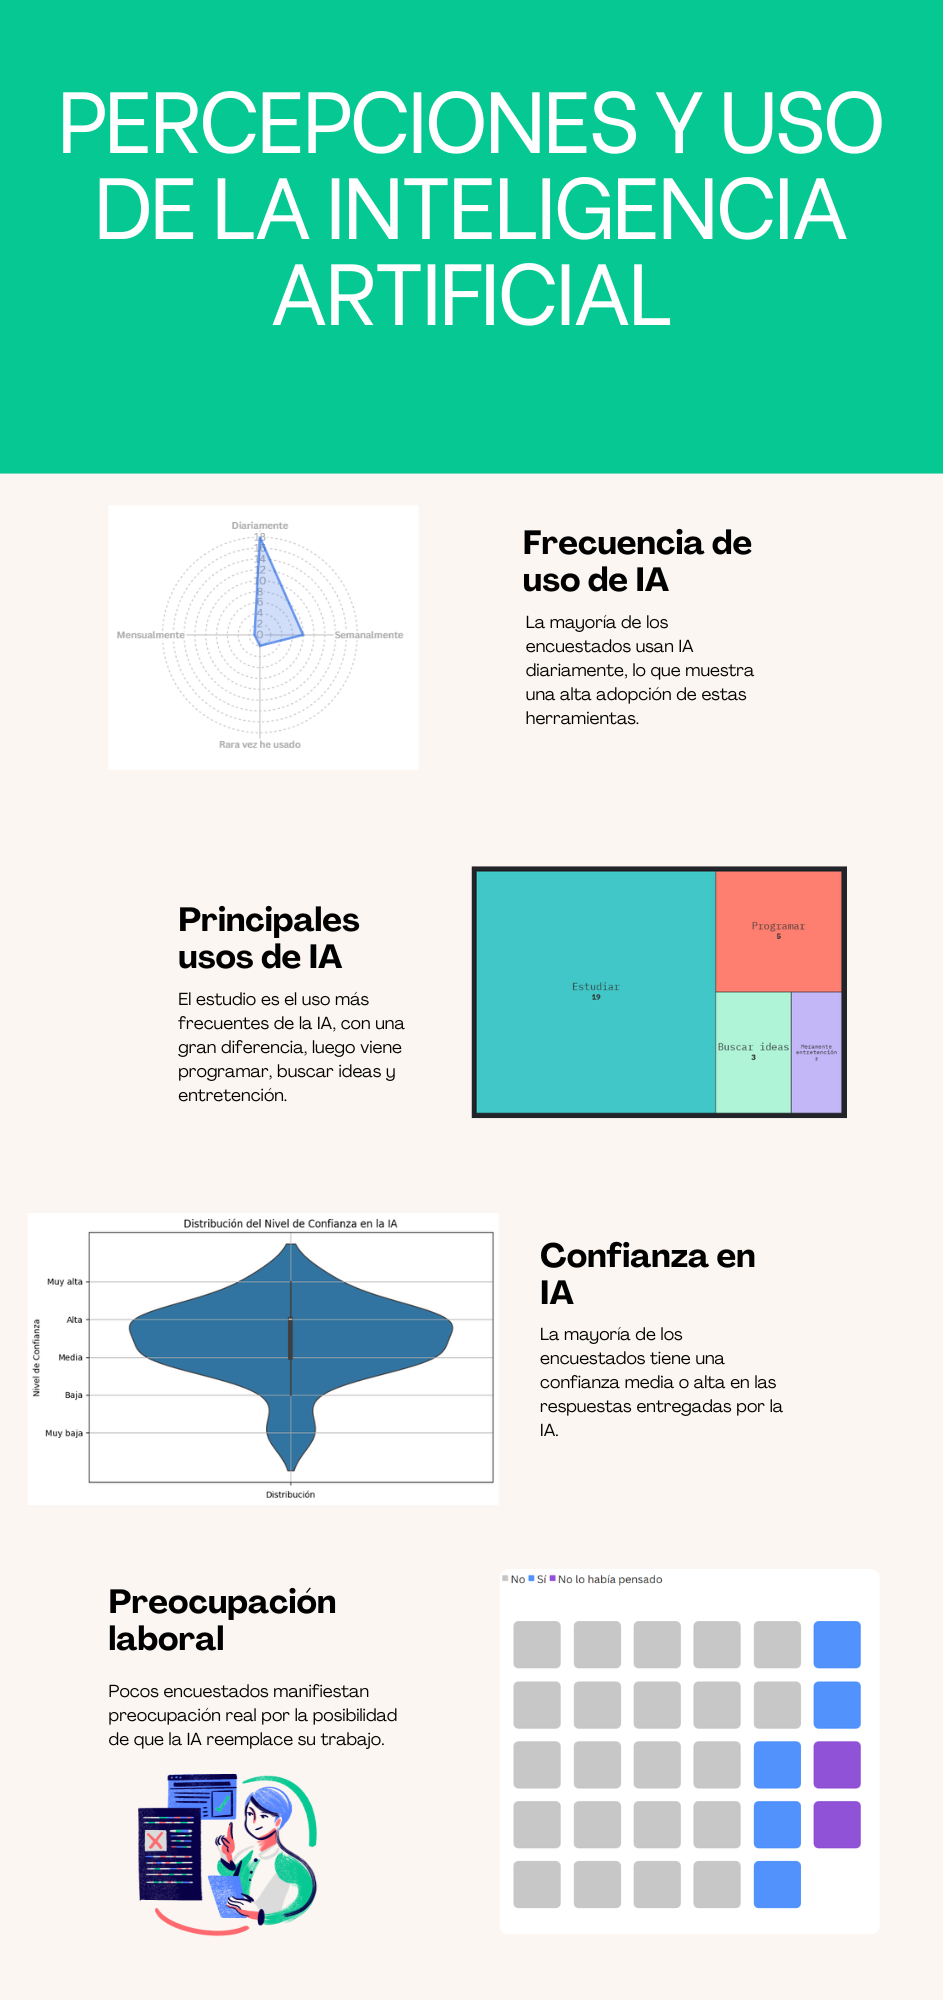
\includegraphics[width=\linewidth]{Graficos/1.png}
        \caption{Primera parte de la infografía: uso, confianza y preocupación}
    \end{minipage}
    \hfill
    \begin{minipage}[t]{0.45\linewidth}
        \centering
        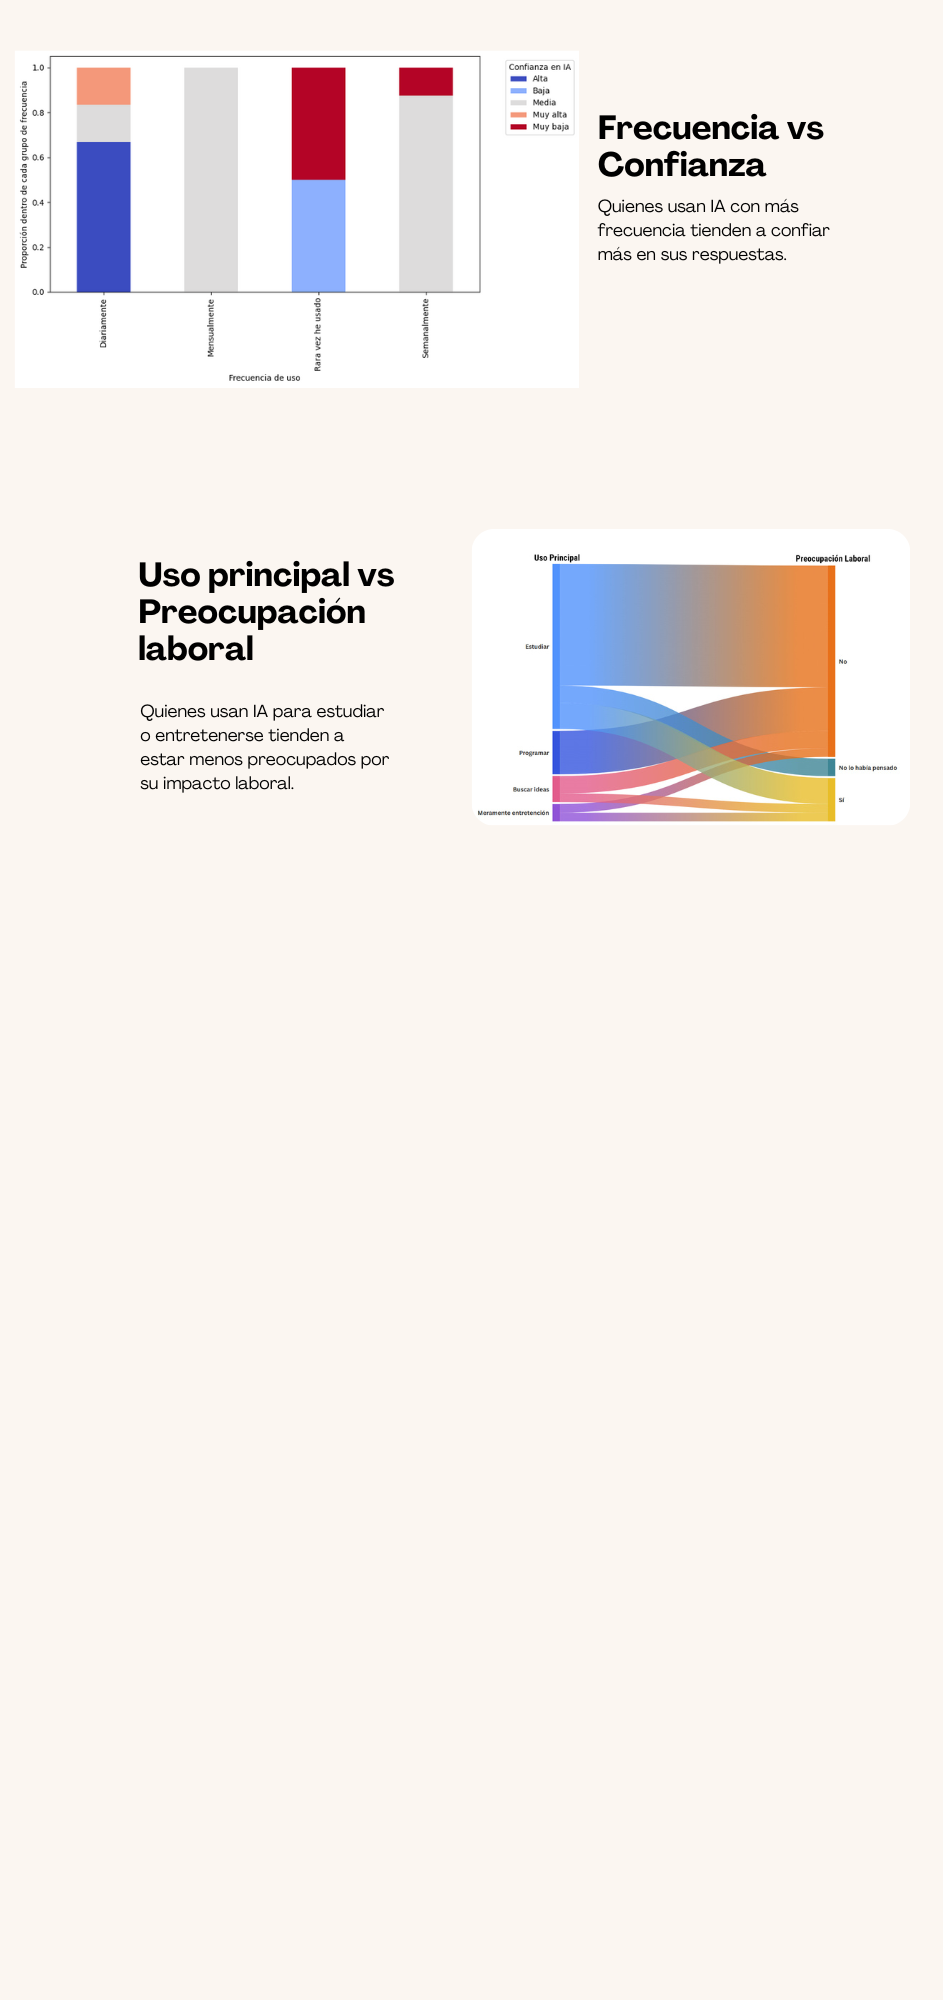
\includegraphics[width=\linewidth]{Graficos/2.png}
        \caption{Segunda parte de la infografía: cruces de variables y percepciones combinadas}
    \end{minipage}
\end{figure}



\section*{Criterios de Selección}
\begin{itemize}
    \item Criterio 1: Principales usos de IA
    \item Criterio 2: Frecuencia de uso de IA	
    \item Criterio 3: Confianza en IA
    \item Criterio 4: Frecuencia vs Confianza
    \item Criterio 5: Preocupación laboral
    \item Criterio 6: Uso principal vs Preocupación laboral	
\end{itemize}

% ---------------------------------------------------------------------------------
\section*{Análisis por Integrante}

% ===================== FELIPE CAMPAÑA =====================
\subsection*{Integrante 1: Felipe Campaña}

\subsubsection*{Criterios Seleccionados}
\begin{itemize}
    \item Frecuencia de uso de IA.
    \item Principales usos de IA.
\end{itemize}

\subsubsection*{Justificación: Principales usos de IA.}
Este indicador muestra los fines más comunes para los cuales se utiliza la inteligencia artificial, como estudiar, crear arte, buscar ideas o programar.

\begin{itemize}
    \item Ayuda a identificar el enfoque funcional que los usuarios dan a la IA en su vida cotidiana.
    \item Refleja cómo las personas aprovechan estas herramientas en contextos académicos, creativos o recreativos.
    \item Es clave para entender el tipo de valor que los usuarios perciben en estas tecnologías.
\end{itemize}

\subsubsection*{Justificación: Frecuencia de uso de IA.}
Este indicador representa la regularidad con la que las personas usan herramientas con inteligencia artificial en su vida diaria, desde un uso esporádico hasta un uso intensivo.

\begin{itemize}
    \item Permite medir el nivel de exposición tecnológica y familiaridad de los usuarios con la IA.
    \item Da cuenta del grado de integración de estas herramientas en rutinas personales o académicas.
    \item Es útil para interpretar otras variables como confianza, percepción o utilidad de la IA.
\end{itemize}


\subsubsection*{Gráfico 1:  Principales usos de IA.}
\begin{figure}[H]
    \centering
    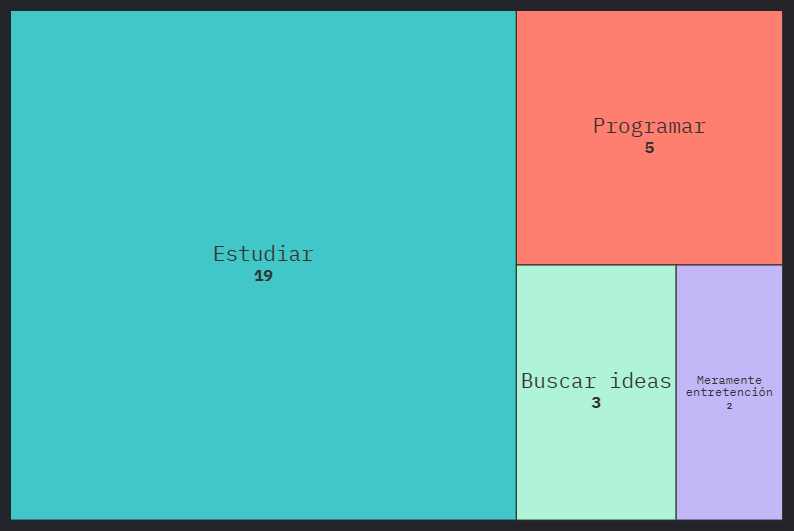
\includegraphics[width=0.85\textwidth]{Graficos/Treemap_Uso_IA_FC.png}
    \caption[1]{Fuente: Elaboración propia con datos}
\end{figure}

\textbf{Conclusión:}
\begin{itemize}
    \item La mayoría de los encuestados utiliza la IA principalmente para estudiar (65\% del total).
    \item Los usos relacionados con programación (17\%) y búsqueda de ideas (10\%) ocupan el segundo y tercer lugar.
    \item El uso recreativo o de entretención representa una minoría (7\%), lo que indica un enfoque más académico o productivo.
    \item El gráfico evidencia que la IA es percibida como una herramienta funcional más que como una distracción.
\end{itemize}

\subsubsection*{Gráfico 2: Frecuencia de uso de IA.}
\begin{figure}[H]
    \centering
    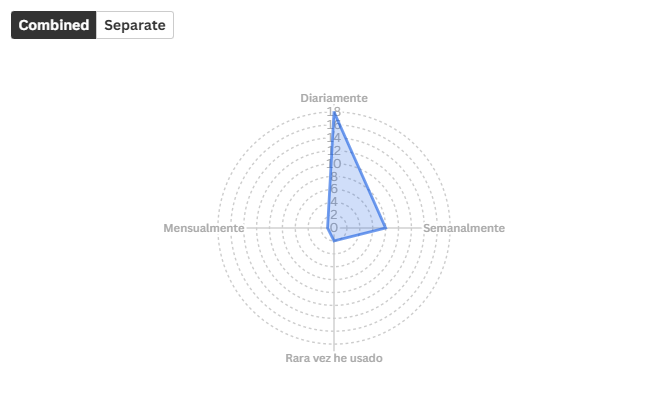
\includegraphics[width=0.85\textwidth]{Graficos/Radar_frec_ia_FC.png}
    \caption[2]{Fuente: Elaboración propia con datos}
\end{figure}

\textbf{Conclusión:}
\begin{itemize}
    \item El uso diario de IA destaca significativamente, representando la categoría con mayor frecuencia entre los encuestados.
    \item El uso semanal también es relevante, aunque menor en comparación con el uso diario.
    \item El gráfico sugiere una integración intensiva de la IA en las rutinas diarias de los participantes.
    \item Esto puede reflejar tanto una alta dependencia como una adaptación natural al uso frecuente de estas tecnologías.
\end{itemize}


% ===================== JAVIER GÓMEZ =====================
\newpage
\subsection*{Integrante 2: Javier Gómez}

\subsubsection*{Criterios Seleccionados}
\begin{itemize}
    \item Criterio 3: Confianza en IA
    \item Criterio 4: Frecuencia vs Confianza
\end{itemize}

\subsubsection*{Justificación: }

\begin{itemize}
    \item El índice de confianza en la IA es importante para comprender cómo el público percibe las tecnologías de éstas mismas, una mayor confianza se asocia con mayores tasas de aprobación de la IA. Además, 
    comprender estos niveles puede ayudar a identificar áreas de mejora en el diseño e implementación de la IA, como la transparencia y la seguridad. 
    Esta información puede ayudar a segmentar a los usuarios según su nivel de confianza y a desarrollar estrategias personalizadas para impulsar la adopción en el uso.
    \item Por otro lado, el criterio de frecuencia versus confianza ayuda a determinar si el uso frecuente de la IA genera una mayor confianza en ella o si, a pesar de su uso constante, los usuarios siguen siendo cautelosos. 
    Si la confianza no aumenta con la frecuencia de uso, puede ser una señal de que los usuarios necesitan más educación o apoyo.
\end{itemize}


\subsubsection*{Gráfico 3: }
\begin{figure}[H]
    \centering
    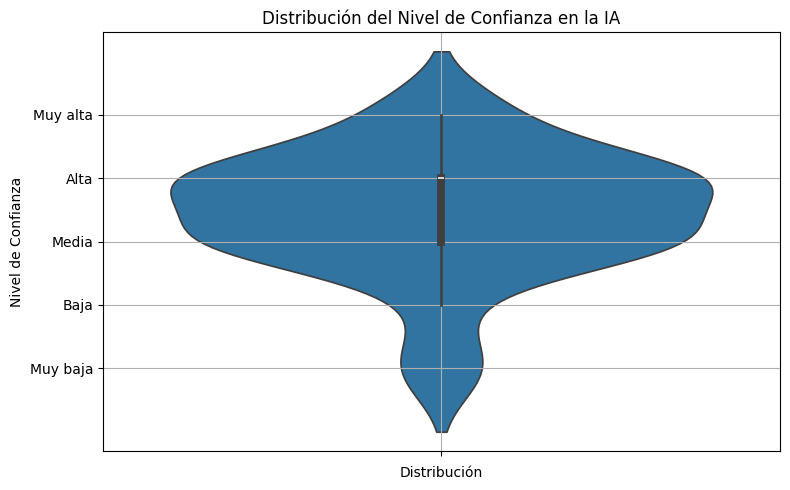
\includegraphics[width=0.85\textwidth]{Graficos/beeswarn.png}
    \caption[3]{Fuente: Elaboración propia con datos}
\end{figure}

\newpage
\textbf{Conclusión:}  
El gráfico sugiere que, en este grupo de 30 personas, la confianza en las respuestas de IA es variada, con posible predominio de posturas moderadas. Esto refleja la complejidad de un tema aún en evolución, 
donde la percepción depende de múltiples factores individuales y contextuales. Seria interesante extrapolar la investigación hacia grupos mas diferenciables para determinar si la edad u profesión podrían llegar a ser un
factor que determine el nivel de confianza que se tenga en las respuestas otorgadas por la IA, por ejemplo los datos recolectados fueron principalmente universitarios, el cual la mayoría presenta un contexto similar.

\subsubsection*{Gráfico 4: }
\begin{figure}[H]
    \centering
    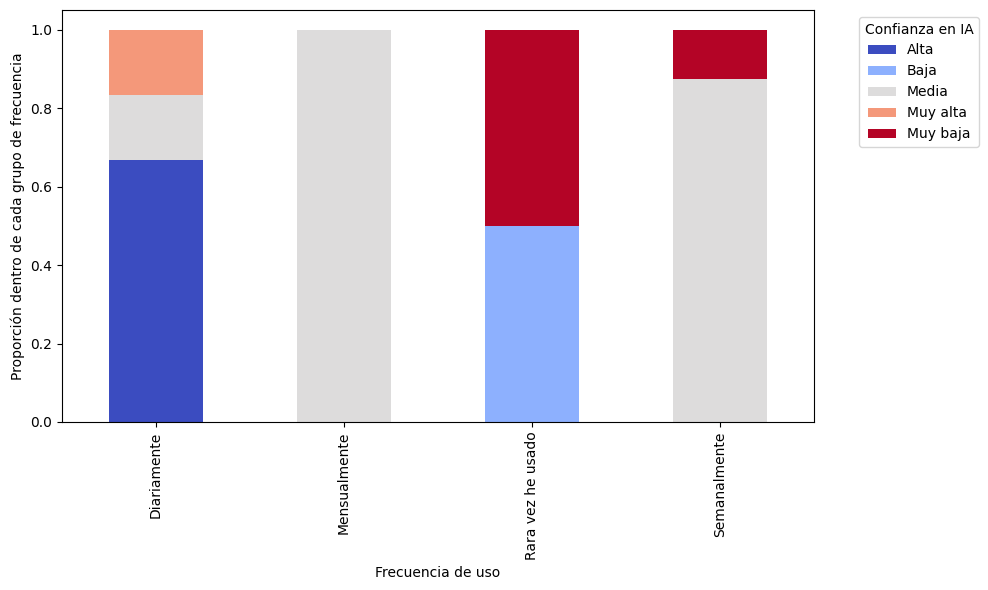
\includegraphics[width=0.85\textwidth]{Graficos/spin plot.png}
    \caption[4]{Fuente: Elaboración propia con datos}

\end{figure}


\textbf{Conclusión:} 
\begin{itemize}
    \item Los valores más altos podrían corresponder a \textbf{Alta}, pero no a \textbf{Muy alta}, lo que refleja un escepticismo generalizado incluso entre usuarios frecuentes.

    \item El gráfico sugiere que la frecuencia del uso de IA aumenta con la confianza que se tiene a esta misma, pero persisten reservas incluso entre usuarios habituales. Esto subraya la necesidad de educación tecnológica y diseño de sistemas de IA más transparentes para cerrar la brecha de confianza.
\end{itemize} 


% ===================== MATÍAS ELGUETA =====================
\subsection*{Integrante 3: Matías Elgueta}

\subsubsection*{Criterios Seleccionados}
\begin{itemize}
    \item Criterio 1: Preocupación laboral ante el avance de la inteligencia artificial
    \item Criterio 2: Relación entre uso principal de IA y preocupación laboral
\end{itemize}

\subsubsection*{Justificación: Preocupación laboral ante el avance de la inteligencia artificial}
Nos permite observar el nivel de preocupación de las personas frente a la posibilidad de que la inteligencia artificial reemplace nuestros trabajos en el futuro. Esta información puede ser útil para:

\begin{itemize}
    \item Analizar tendencias de los encuestados ante la pregunta planeada con el objetivo de no dejar de lado la opinión de la mayoría.
    \item Diseñar estrategias de comunicación que aborden los temores asociados a la automatización, fomentando una transición tecnológica más informada y segura para los trabajadores.
\end{itemize}

\subsubsection*{Justificación: Relación entre uso principal de IA y preocupación laboral}
Nos permite analizar cómo se relaciona el propósito principal del uso de la inteligencia artificial con la preocupación por el reemplazo laboral, lo cual aporta una visión más segmentada del impacto percibido de esta tecnología. Esto puede ser útil para:
\begin{itemize}
    \item Comprender si quienes utilizan IA con fines productivos (como programación o estudio) tienen percepciones distintas respecto a su impacto laboral, lo que puede orientar campañas diferenciadas de formación o comunicación.
    \item Anticipar patrones de adopción y resistencia tecnológica en distintos grupos, facilitando la planificación de políticas laborales o educativas adaptadas al nivel de exposición y percepción de riesgo frente a la IA.
\end{itemize}

\subsubsection*{Gráfico 5: Preocupación laboral ante el avance de la inteligencia artificial}
\begin{figure}[H]
    \centering
    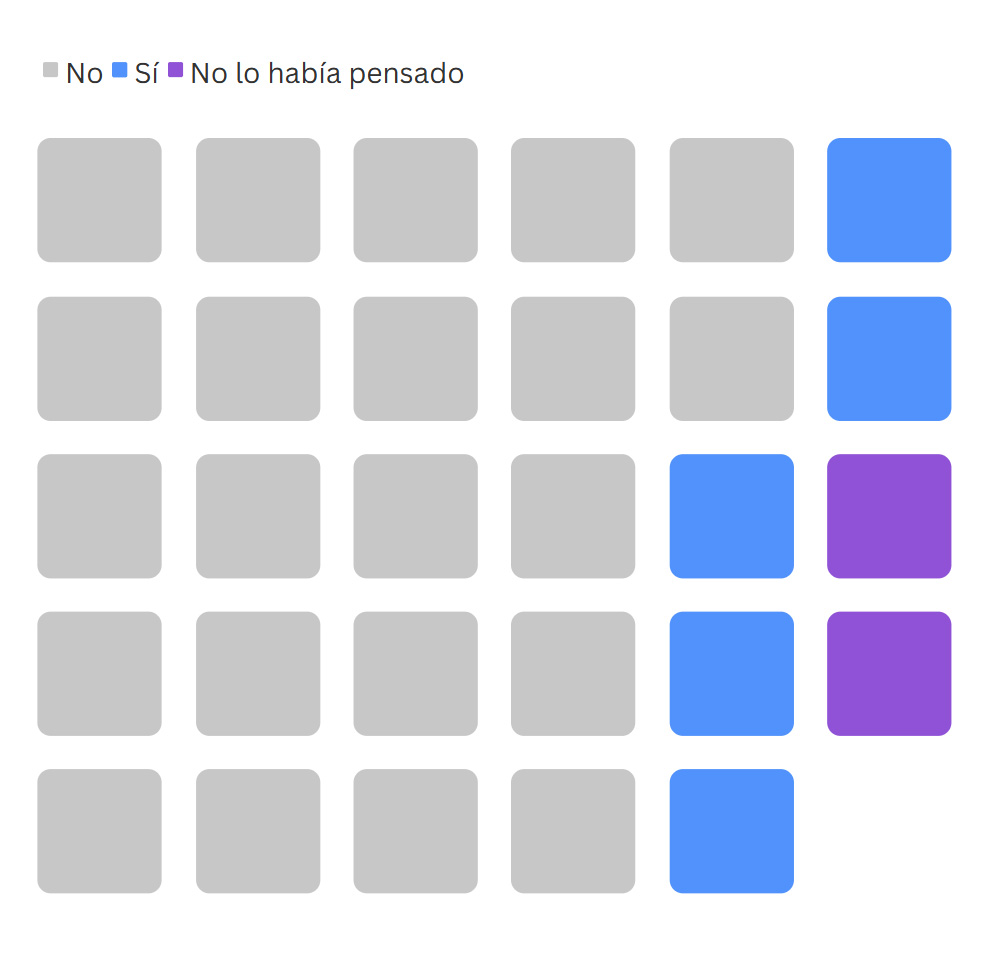
\includegraphics[width=0.85\textwidth]{Graficos/PreocupacionLaboral.jpg}
    \caption[5]{Fuente: Elaboración propia con datos}
\end{figure}

\textbf{Conclusión:}  
\begin{itemize}
    \item Se observa que la gran mayoría de los encuestados no manifiesta preocupación respecto a que la inteligencia artificial reemplace sus trabajos, con 22 de 29 personas (76\%) seleccionando la opción "No".
    \item Un grupo reducido expresa preocupación explícita (5 personas) o una reflexión tardía al respecto (2 personas que no lo habían pensado), lo cual indica que, si bien el tema existe en el imaginario colectivo, aún no representa una alarma generalizada entre los participantes.
    \item Esta distribución puede interpretarse como una señal de confianza en la propia adaptabilidad profesional o una falta de conciencia sobre los posibles impactos laborales de la automatización.
\end{itemize}

\subsubsection*{Gráfico 6: Relación entre uso principal de IA y preocupación laboral}
\begin{figure}[H]
    \centering
    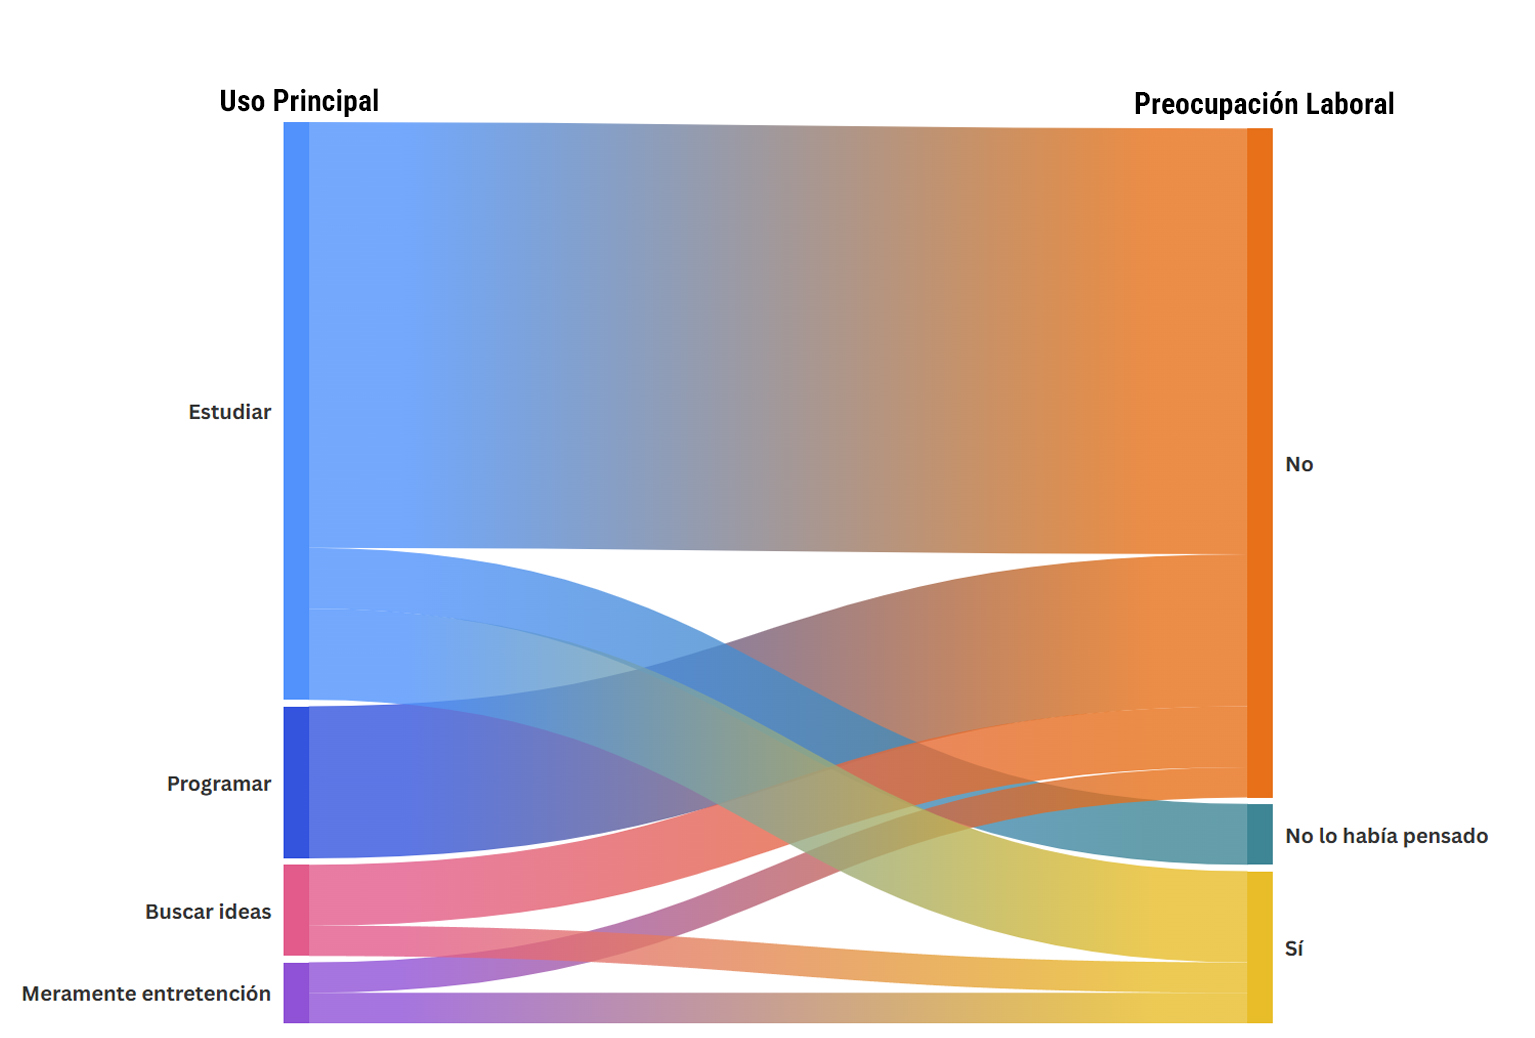
\includegraphics[width=0.85\textwidth]{Graficos/UsoPrincipalVSPreocupacionLaboral.jpg}
    \caption[6]{Fuente: Elaboración propia con datos}

\end{figure}


\textbf{Conclusión:}  
\begin{itemize}
    \item El gráfico Sankey revela que los encuestados que utilizan IA principalmente para estudiar presentan una mayor diversidad de respuestas respecto a la preocupación laboral, siendo el único grupo con representación significativa en las tres categorías: “Sí”, “No” y “No lo había pensado”.
    \item En contraste, todos quienes usan IA principalmente para programar afirman no estar preocupados por su posible reemplazo laboral, lo que podría deberse a una mayor familiaridad técnica o confianza en el valor agregado de sus habilidades.
    \item Aquellos que emplean IA para buscar ideas o con fines de entretenimiento muestran un patrón menos claro, pero igualmente destacan por tener menor nivel de preocupación, reforzando la idea de que el tipo de uso influye en la percepción del riesgo asociado al avance de la IA.

\end{itemize}

% ---------------------------------------------------------------------------------}
\section{Evidencia de encuesta aplicada}

A continuación, se presenta una imagen del archivo en Excel que contiene las respuestas recolectadas de la encuesta sobre el uso de inteligencia artificial. Esta tabla incluye los datos utilizados para generar los gráficos presentados anteriormente. Se realizo en google forms para mayor comodidad y cantidad de respuestas. 

\begin{figure}[H]
    \centering
    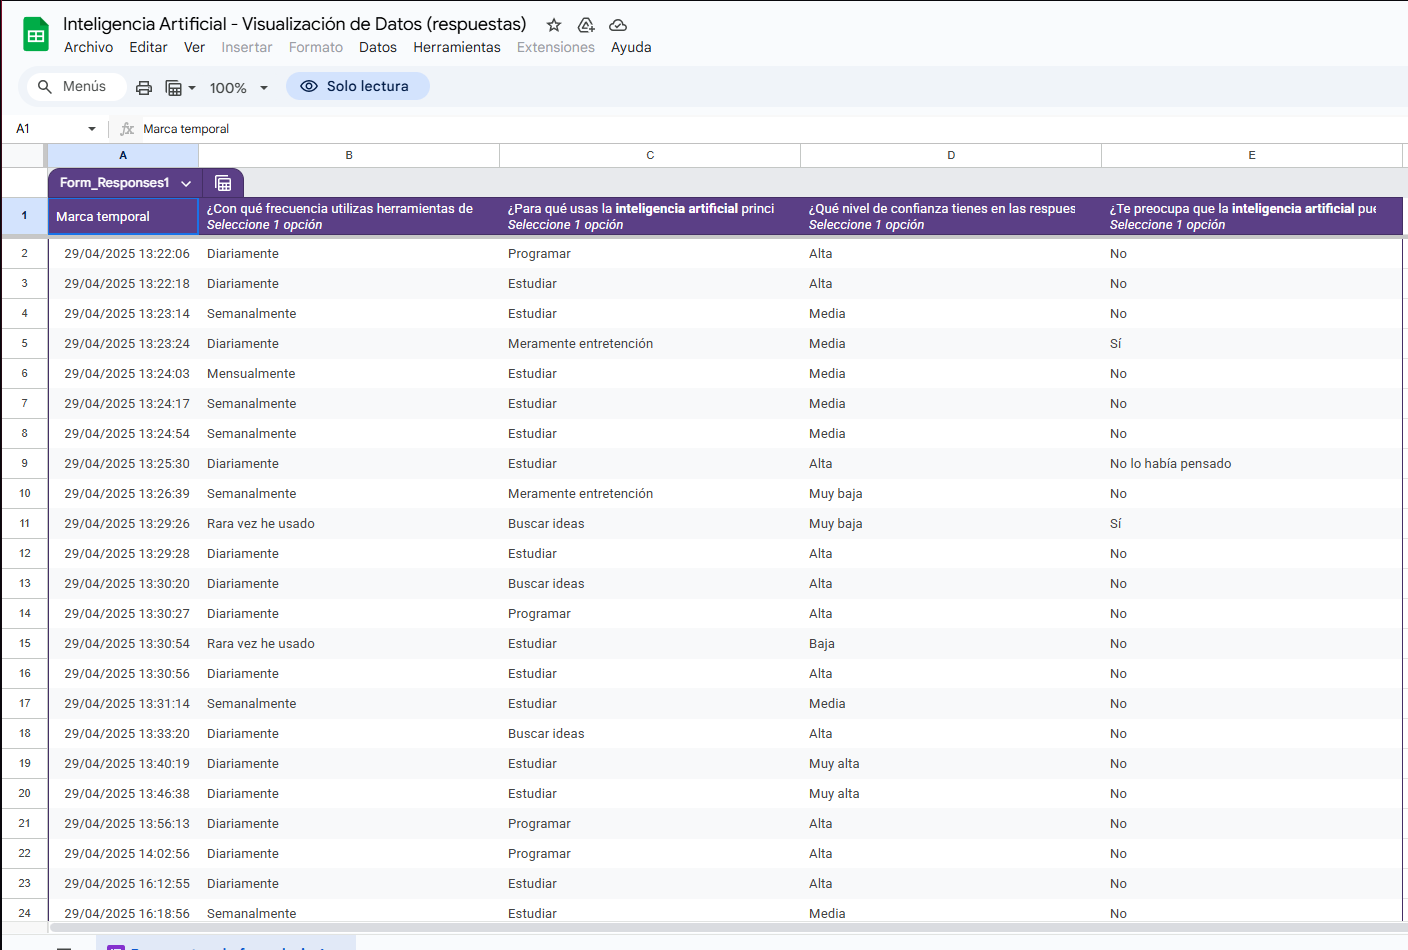
\includegraphics[width=0.95\textwidth]{Graficos/excel.png} % <-- nombre del archivo imagen
    \caption{Captura de pantalla del archivo Excel con las respuestas de la encuesta}
\end{figure}

El archivo completo puede ser consultado en el siguiente enlace:

\begin{itemize}
    \item \href{https://docs.google.com/spreadsheets/d/1KRdGL7pflDiA8TAT_pvPSt6OpXGPv6h4NTGceC8xDS0/edit?resourcekey=&gid=168064728#gid=168064728}{Ver archivo Excel de la encuesta}
\end{itemize}


\textbf{Repositorio:}  
\label{anexo:repositorio}

Acceso al repositorio en el siguiente link: 
\url{https://github.com/soloimsad/VD.git}

\end{document}